%\begin{figure}[t]
%
%   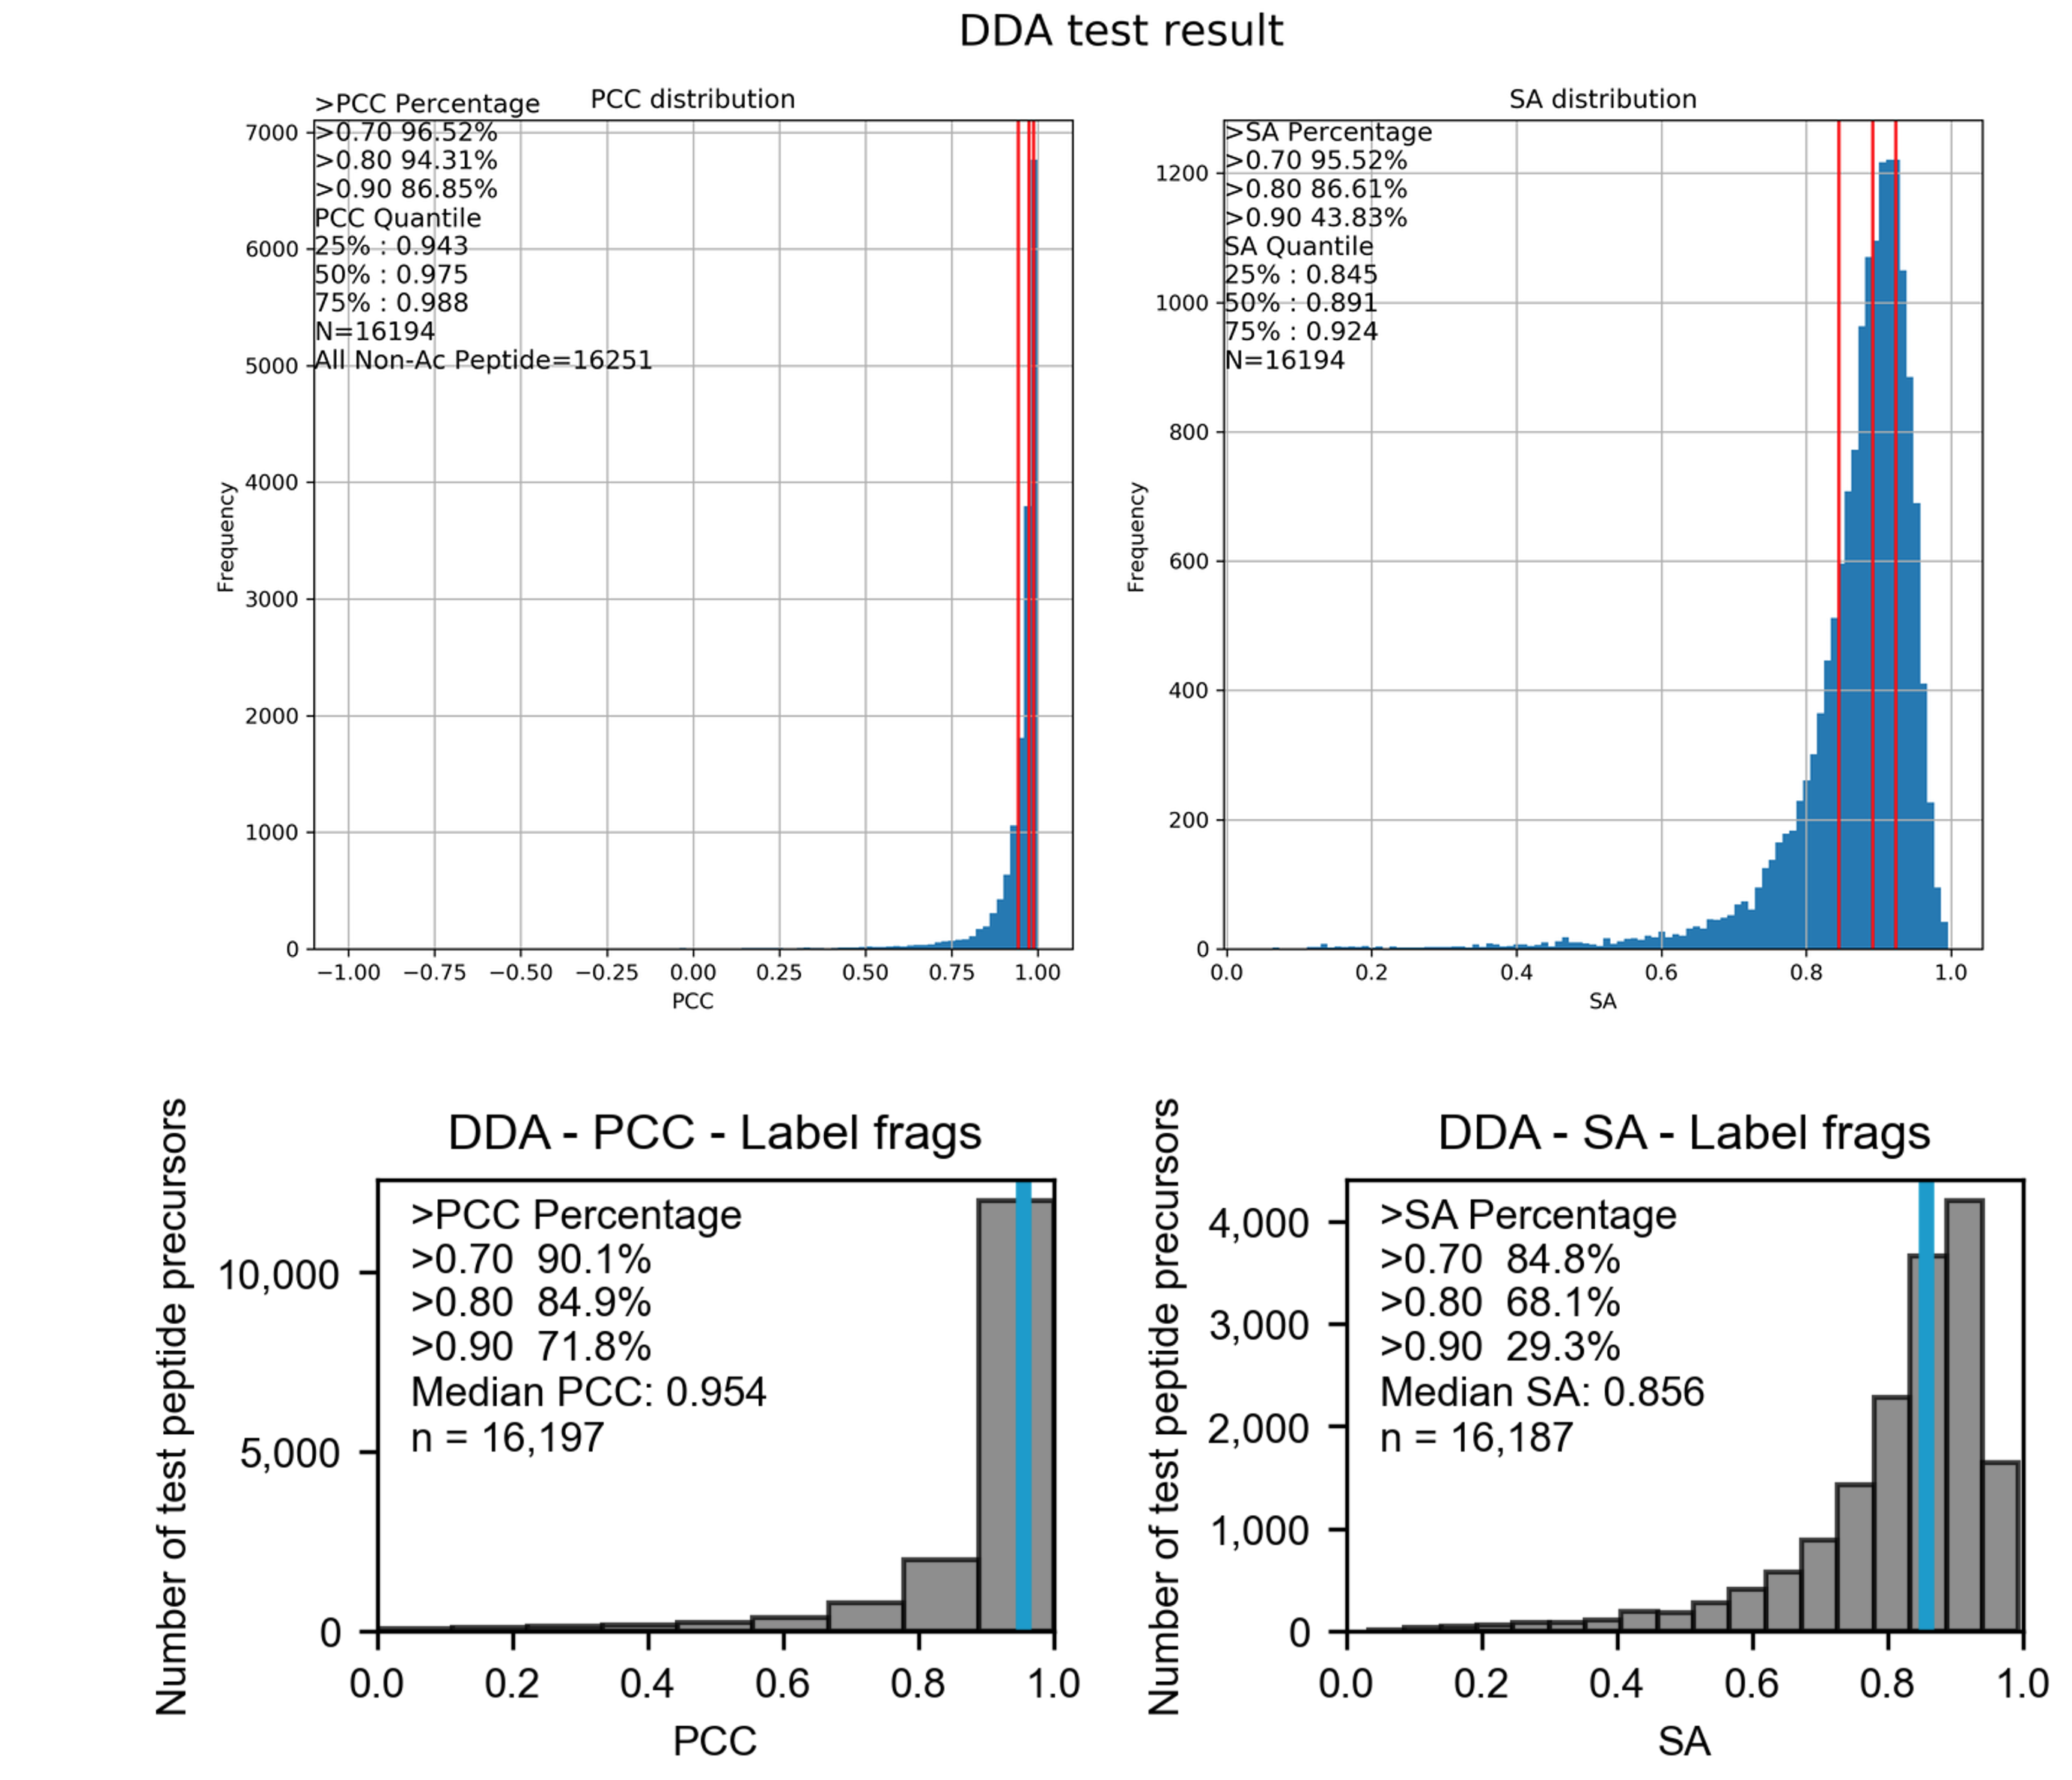
\includegraphics[width=3.0in]{DDA}
%
%   \caption{Visualization of performance of DDA dataset. The above is ours and the below is pdeep2}
%\label{fig:DDA}
%\end{figure}
%
%
%\begin{figure}[t]
%
%   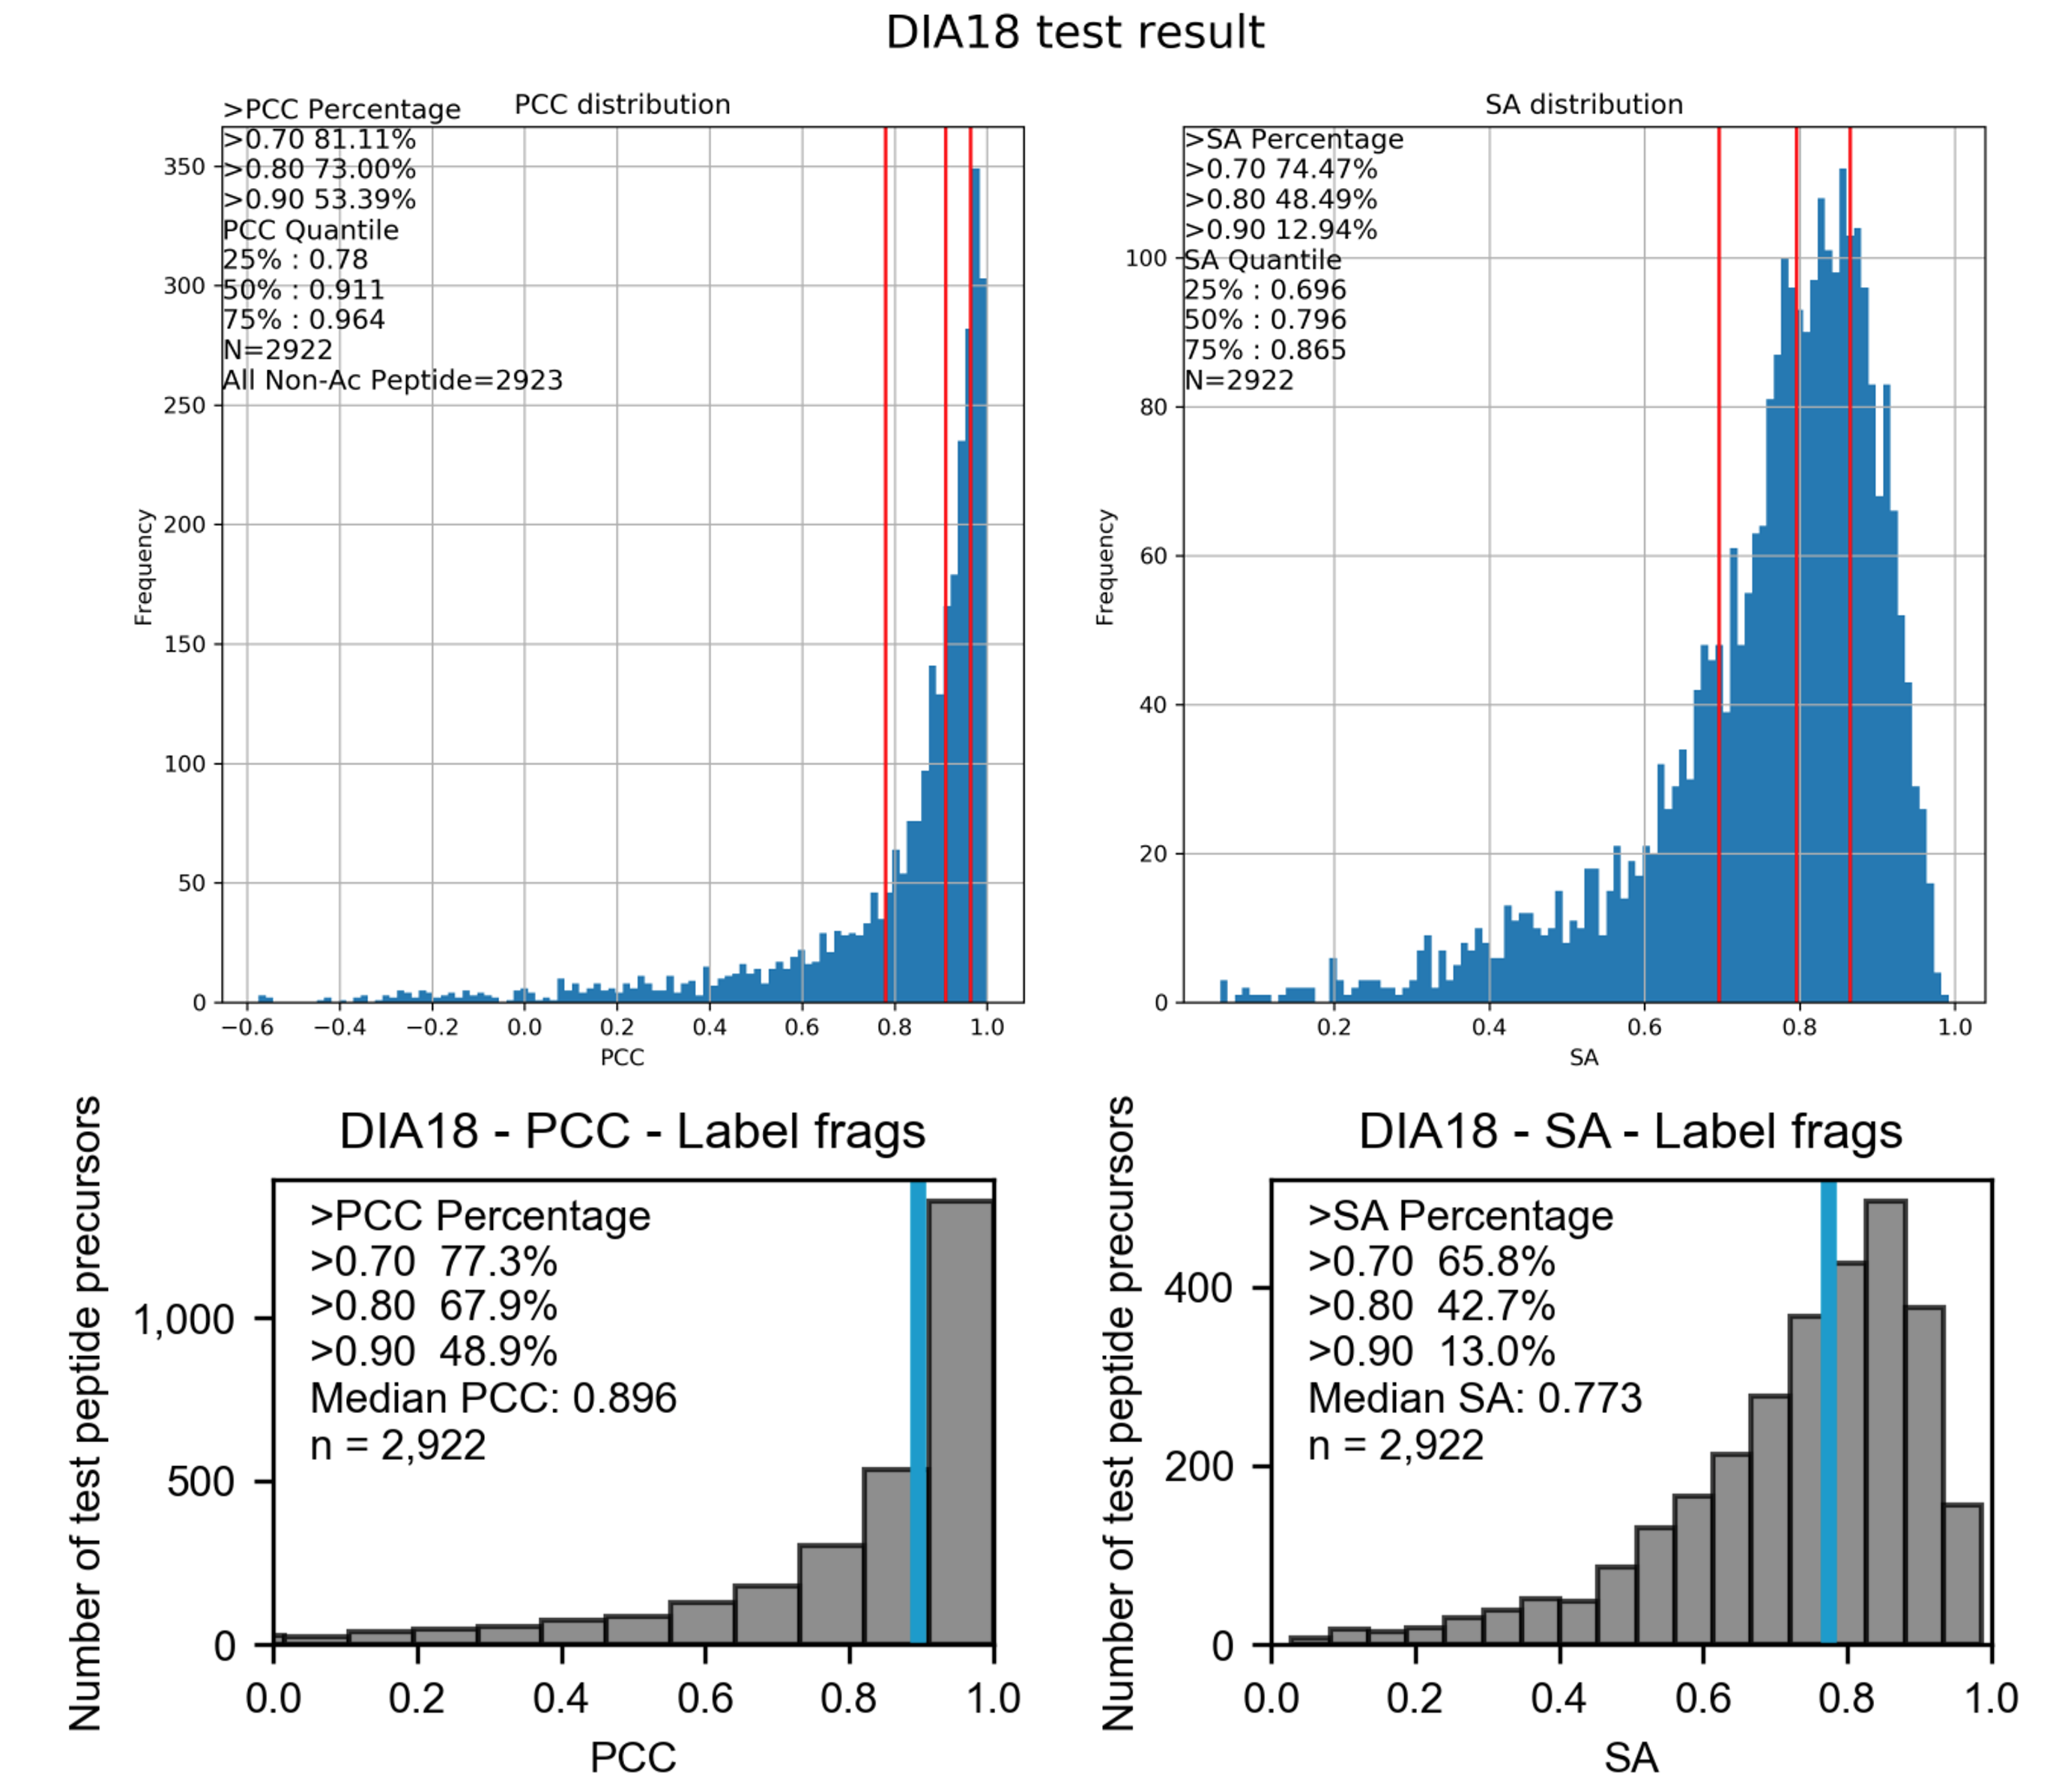
\includegraphics[width=3.0in]{DIA18}
%
%   \caption{Visualization of DIA18 dataset. The above is ours and the below is pdeep2}
%\label{fig:DIA18}
%\end{figure}
%
%



\begin{table}
   \begin{center}
   \begin{tabularx}{\columnwidth}{|m{0.4\columnwidth}|Y|Y|}
   \hline
   data description & no. of peptides & no. of spectra\\
   \hline
   HumanPhosDB~\cite{lawrence2016plug} & 204,558 & -\\
   Jeff~\cite{liu2018vivo} & 67,552 & 89,437\\
   VeroE6~\cite{bouhaddou2020global} & 43,405  & 54,004\\
   R2P2~\cite{leutert2019r2} & 35,808 & 43,312\\
   U2OS-DIA~\cite{wang2020naguider} & 48,327 & 58,843\\
   RPE1-DIA~\cite{bekker2020rapid} & 33,576 & 39,977\\
   RPE1-DDA~\cite{bekker2020rapid} & 129,109 & 165,719\\
   \hline
   \end{tabularx}
   \end{center}
   \caption{Retention time datasets}
   \label{table:Datasets}
\end{table}

\begin{table}
  \begin{center}
  \resizebox{\columnwidth}{!}$ where the lower is the better, and the right is PCC where the higher is the better.}
  \label{table:RT results}
\end{table}

\begin{table}
  \begin{center}
  \resizebox{\columnwidth}{!}{%
  \begin{tabular}{|c|c|c|c|}
  \hline
  method & U2OS-DIA & RPE1-DIA & RPE1-DDA\\
  \hline\hline
  pDeep2 & 0.887/0.778 & 0.867/0.767 & 0.954/0.855 \\
  \hline
  \textbf{DeepPhospho} & \textbf{0.915}/\textbf{0.804} & \textbf{0.903}/\textbf{0.791} & \textbf{0.968}/\textbf{0.881} \\
  \hline
  \end{tabular}
  }
  \end{center}
  \caption{Ion Intensity Dataset results. The left number in cell is median PCC and the right is median SA where the higher is the better for both metrics.}
  \label{table:Ion Intensity results}
\end{table}

\begin{table}
   \begin{center}
   \begin{tabularx}{\columnwidth}{|m{0.35\columnwidth}|Y|Y|}
   \hline
   model & Median PCC & Median SA\\
   \hline
   w/o LSTM & 0.949 & 0.834 \\
   w/o Transformer & 0.951 & 0.835\\
   CNN-Transformer & 0.949  & 0.839\\
   \textbf{DeepPhospho} & \textbf{0.955} & \textbf{0.844}\\
   \hline
   \end{tabularx}
   \end{center}
   \caption{Ablation study on Jeff dataset}
   \label{table:ablation study}
\end{table}